\emph{Das Kapitel Methoden ermöglicht es anderen, deine Ergebnisse zu reproduzieren, ohne den Abschnitt Ergebnisse zu lesen. 
Hier beantwortest du also Fragen wie:
\begin{itemize}
\item Wie entwirfst du dein Gerät oder deinen Controller? % Letzteres könnte z. B. in einem Unterabschnitt {Control Design} untergebracht werden.
\item Wie entwirfst du Experimente oder Simulationen? % Experimentprotokoll
\item Wie sammelst und analysierst du die Daten? % Z.B. \Unterabschnitt{Datenerfassung}, \Unterabschnitt{Datenanalyse}
\end{itemize}
Wähle beschreibende Namen für neue Methoden (anstelle von Wörtern wie "Neuheit"), um die Zitierung und künftige Verbesserungen zu vereinfachen.}

%--------------------------------------------------------
\section*{ Was bedeutet wissenschaftliches Schreiben?}

Wissenschaftliches Schreiben vermittelt \cite{simbeck_etal}
sehr gut. Hier findest Du Selbstlernmaterialien für Abschlussarbeiten, aber auch für Hausarbeiten und Labor-/ Versuchsprotokolle. 

%---------------------------------------------------------

\subsection{Formulieren}
\label{sec:writing}

\begin{itemize}
	\item Vermeide Rechtschreib- und Zeichensetzungsfehler. 
     \item Schreibe in kurzen und prägnanten Sätzen. 
	\item Vermeide die Verwendung der ersten Person (``ich'' und ``wir'').
	\item Verwende keine Verkürzungen oder umgangssprachliche Formulierungen.
    \item Vermeide Wortwiederholungen. Berücksichtige jedoch: In wissenschaftlich technischen Bereich sind Fachbegriffe oft eng umgrenzt. Daher kann die Verwendung von unterschiedlichen Fachbegriffen für einen speziellen Sachverhalt zu Missverständnissen führen. 
    \item Vermeide ungebräuchliche Abkürzungen, und zwar auch dann, wenn diese in deiner Dokumentation explizit erklärt werden. 
\end{itemize}

\paragraph{Und in englischer Sprache}
\emph{
\begin{itemize}
	\item  Do not use contractions (don't) or colloquial speech.
    \item  Avoid static verbs and passive tense; try to write actively. As an exercise, start by replacing all forms of ``to be'' in your first two paragraphs with an active construction. %(just replacing the word, with terms like ``exist'', does not make it better).
    \item  Look up the rules for hyphenation in English, particularly for ``compound modifiers'', to know the difference between a ``red haired person'' and a ``red-haired person''.
    \item  Look up the rules for which/that (including punctuation).
    \item  Whenever you look something up (like grammar rules), do not trust newsgroups or other sources like that. Get a reliable source, e.g. a book.
    \item  Try to use only English words you know! 
    \item  \href{https://www.merriam-webster.com/}{Merriam-Webster} helps with spelling and hyphenation.
\end{itemize}}

%-----------------------------------------------------
\subsection{Darstellen von Abbildungen und Tabellen}
\label{sec:bildertabs}

Eigene Abbildungen können durch Fotos, durch echtes Texen, durch eigenhändiges Zeichnen und digitalisieren des Bildes oder das Erstellen einer Grafik in einem Grafikprogramm entstehen. 

\begin{itemize}
    \item Scheue nicht den Aufwand einer sinnvollen Abbildung. Sie liefert oft deutlich bessere Erklärungen als verbale Beschreibungen von Sachverhalten
    \item Verweise auf alle Abbildungen und Tabellen im Text, bevor sie erscheinen. Beispiel: Die Sprungantwort des Systems zeigt ein zeitverzögertes Verhalten erster Ordnung... (Abb.~\ref{fig:boxplot}).
    \item Verwende nach Möglichkeit Vektorgrafiken; raster den Text nicht. Du kannst Abbildungen als \texttt{.eps} aus Matlab exportieren.
    \item Vergewissere dich, dass deine Abbildungen im Schwarzweißdruck und von Farbenblinden perfekt lesbar sind. Verwende also nicht (nur) Farbcodes, sondern auch unterschiedliche Linienstile, Dicken oder Graustufen.
    \item Der gesamte Text in den Abbildungen sollte ohne Zoom lesbar sein. Verwende daher keine Schriftgrößen, die kleiner als die Fußnotengröße sind. 
    \item Verwende für Symbole in Abbildungen die gleiche Schriftart wie im Haupttext. Ein Paket, das hier hilft, ist \texttt{psfrag}. Es ersetzt während der Kompilierung den Text in deinen Abbildungen durch Text oder Variablen deiner Wahl. %Bemerkung: Wenn Sie Illustrator verwenden, funktioniert das Paket am besten, wenn Sie eine Version Ihrer Datei in einem älteren Format (z. B. Illustrator 3) speichern. 
    \item In Tabellen und Abbildungen gelten die in Abschnitt {sec:formulas} genannten Regeln für den Formelsatz. Bei Beachtung der Regeln ergeben sich drei formal korrekte Beschriftungen von Koordinatensystemen in Diagrammen.
    
\begin{figure}[h!]
\psfrag{#Wd}[lc][lc]{\sffamily\small  Führungsgröße $w(t)$}
\psfrag{xa}[t][c]{$F$/N}
\psfrag{ZIm}[t][b]{$A$}
\psfrag{Elast}[t][b]{\sffamily  B}
\psfrag{Com}[t][b]{ $C$}
\psfrag{5}[r][r]{\sffamily  5}
\psfrag{10}[r][r]{10}
\psfrag{15}[r][r]{$15$}
\psfrag{20}[r][r]{\sffamily 20}
\centering
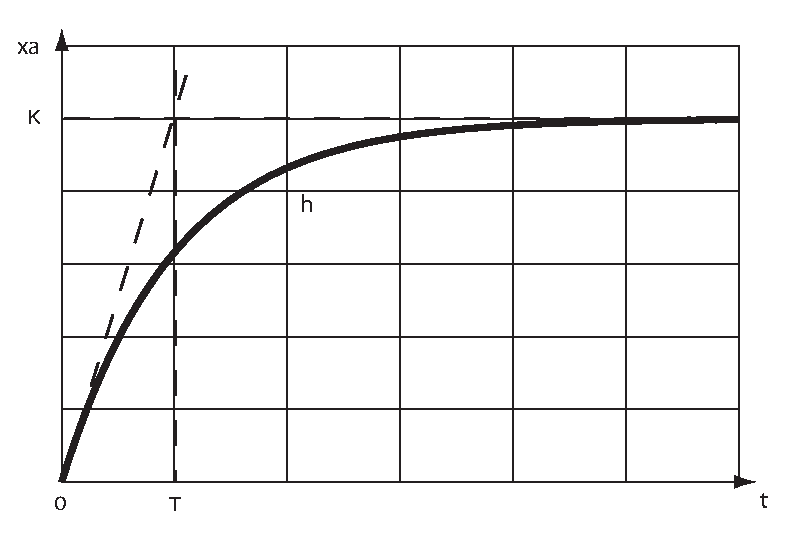
\includegraphics[width=0.9\textwidth]{figures/step_pt1.eps}
\caption[Boxplot]{Diese Abbildung zeigt eine Matlab-Darstellung, exportiert nach eps Force $F$ für die Bedingungen $A$, $B$, und $C$. {Beispiele für korrekte Achsenbeschriftungen, Beispiel für formal falsche Achsenbeschriftung}}
\label{fig:boxplot}
\end{figure}

 \begin{figure}
    \centering
    \begin{tikzpicture}
	\begin{axis}[
    	xlabel=$t$ in s,
        ylabel=$v$ in $\frac{\mathrm{rad}}{\mathrm{s}}$,
		no marks,
		line width = 1pt,
		grid,
		width=12cm,
		height=5cm,
		xmin=0.5,
        xmax=5,
		legend pos=outer north east,]
		\addplot table[col sep=comma,y=y1]{template_thesis_htw/vorlage_thesis/PGF/vergleich_sim_real_data.txt};
		\addplot table[col sep=comma,y=y2]{template_thesis_htw/vorlage_thesis/PGF/vergleich_sim_real_data.txt};
		\legend{Real, Simulation}
	\end{axis}
\end{tikzpicture}

    \caption{Vergleich simulations- mit realem Verhalten}
    \label{fig: Vergleich Simulation mit realem verhalten}
\end{figure}

    \item Beim Zeichnen von Blockdiagrammen ist die IEC-Notation~\cite{IECControltech} zu verwenden. Beispiele: Kreise für Summenpunkte verwenden, Vorzeichen an der rechten Seite der eingehenden Aktionslinien positionieren, Punkte für Verzweigungspunkte verwenden, rechteckige Blöcke verwenden.
    \item Zeichnungen sind unter Verwendung genormter Schaltzeichen, Bildzeichen und Symbole anzufertigen und zu beschriften. Zeichenblätter, deren Format größer als DIN~A4 ist, sind gefaltet dem Text beizuheften oder beizulegen.
\end{itemize}

 
Tabellen sind mit Abbildungen vergleichbar, weshalb das zuvor Gesagte weitgehend auch für Tabellen gilt. Genau wie Abbildungen müssen auch Tabellen nummeriert werden. Üblich ist es, für Tabellen eine eigene Nummerierung zu verwenden, d.h. in einer Dokumentation gibt es möglicherweise eine Abbildung 1 und eine Tabelle 1.


\begin{table}[h]
    \centering
   \begin{tabular}{l|rc}
	Semester   &Anzahl betreuter BAs   & Anzahl betreuter MAs\\
    WS20/21     &2      &5\\
    WS20/21     &2      &5\\
    WS20/21     &2      &5\\
\end{tabular}
	\caption{Auflistung der von Prof.~Heide Brandtstädter betreuten Abschlussarbeiten.}
	\label{tab:BAsMas}
\end{table}


%----------------------------------------------------------
\subsection{Formelsatz }
\label{sec:formulas}



\begin{itemize}
\item Definiere jede einzelne Variable explizit. Verlasse dich nicht auf ``selbsterklärende'' Indizes wie $x_{\mathrm{max}}$ oder auf den Erfahrungshintergrund des Lesers (z.B. um anzunehmen, dass $I$ ein elektrischer Strom sein muss). Wähle kurze Indizes, lieber einen als mehrere Buchstaben. 
	\item Benutze keinen Operator zwischen Variablen, oder ``$\cdot$'' wenn nötig. Beispiel: $F=ma=\,{3}{kg}\cdot\,{2}{m/s^2}$.

\item Es bietet sich an besondere Zeichensetzung die nicht direkt eindeutig ist entsprechend zu kennzeichnen z.B.
\begin{equation}
    \cA \prec 0
\end{equation}
hier soll $\prec$ zeigen, dass die Matrix $\cA$ negativ definit ist. 

\item Beginne Sätze nicht mit Zahlen oder Variablennamen. Manchmal hilft es, Konstruktionen wie ``Der Parameter $k$'' oder ``Die Variable $x$'' oder ``Ein Wert von 20...'' zu verwenden.

\item Setze Skalare, Vektoren und Matrizen anders. Beispiel:
Die Massenmatrix $M M_{\textnormal{r}}(V{q})$ eines Robotermanipulators ist eine Funktion der verallgemeinerten Koordinaten des Roboters~$V{q}$. Um dies zu aktivieren, verwende z.B.
\begin{verbatim}
\newcommand{\V}[1]{\boldsymbol{#1}}%vectors
\newcommand{\M}[1]{\mathbf{#1}}%matrices
\end{verbatim}
 in der Präambel deines Dokuments.

\item Fügen Sie Formeln in Sätze ein. Setzen Sie Punkte, wenn ein Satz nach Ihrer Gleichung endet, oder ein Komma, wenn es angebracht ist. 
%\item Make formulae part of sentences. Place full stops when a sentence ends after your equation, or a comma when appropriate. See the above example equation \eqref{eq:derivative}. %Another example: $\V{F}=m \V{a}$, with $m$....

% Example for how to reference an equation: With~(\ref{eq:derivative}), ...
\end{itemize}

Die Normen \cite{ISOnormunits}\cite{DINGroessen}\cite{DINFormelsatz}\cite{DINGroessen} 
regeln, welche Buchstaben für Größen und Einheiten zu verwenden und wie Formeln darzustellen sind. Dabei ist auch geregelt, welche Zeichen gerade und welche kursiv zu setzen sowie wo Leerzeichen einzufügen
sind.

\begin{itemize}

\item Operatoren und gängige mathematische Funktionen werden im Hochformat gesetzt~\cite{RedBook2010}. Besonders häufig wird dies bei dem Differentialoperator oder bei sin und cos falsch gemacht. Beispiel: Die Ableitung der Variablen $x$ nach der Zeit $t$ ist
\begin{equation}
\dot{x}=\frac{\d x}{\d t} \, .
\label{eq:derivative}
\end{equation}


Wie in \ref{eq:tolleformel}
\item Die mathematischen Konstanten $\pi$, $e$ und $i$, als auch mathematische Funktionen wie $\sin$, $\cos$, $\tan$, $\lim$, $\ln$, sowie Summen- und Integralzeichen werden gerade gesetzt.

\begin{align}
    \pi^{\frac{2^7}{1+\frac{1}{\Omega}}}\label{eq:tolleformel}
\end{align}

Der Befehl \textbackslash cos\{\} kann hier leicht verwendet werden um trigonometrische Funktionen zu verwenden wie hier demonstriert:

\begin{equation}
    f(x) = \cos{(x)} 
\end{equation}

\item Alles, was Text ist, sollte nicht als Variablen gesetzt werden. Dies gilt auch für Indizes von Variablen. Zum Beispiel, für eine Variable $\lambda$ mit dem beabsichtigten Index ``m'', wobei ``m'' eine Abkürzung für ``max'' ist, schreiben Sie $\lambda_{\mathrm{m}}$ und nicht $\lambda_m$.
\item Beispiel für bezeichnende und variable Indizes
\item Indizes werden gerade gesetzt, wenn sie die Variable näher bezeichnen. Lediglich variable Indizes werden kursiv gesetzt.
\begin{equation}
    a = \sum^{n}_{i=1} b_i
\end{equation}
    \item Variablen und Größen werden kursiv gesetzt
\item Zahlen und Einheiten werden gerade gesetzt
\item Zwischen Variable und Einheit steht immer ein Leerzeichen. 
\item Ausnahme Prozent-Zeichen (\%) kann das Leerzeichen wahlweise stehen oder entfallen.
\item Ausnahme Bei Winkelbezeichnungen und Gradangaben (°) entfällt das Leerzeichen.
Beispiele

\item Chemische Formelzeichen und Abkürzungen werden gerade gesetzt.
\item Einheiten: Es ist ein sehr häufiger Fehler, eckige Klammern um die Einheit zu setzen. Dies ist nach der SI~\cite{SIbrochure2006} und der ISO-Norm~\cite{ISOnormunits} nicht korrekt. Beispiel: Für eine Kraft $F$ ist die korrekte Verwendung des Operators: $[F]=\,{N}$. Für Achsenbeschriftungen in Diagrammen ist die Division wie in ``$F/\,{N}$'' (bevorzugt) oder ``Kraft $F$ (in \,{N})'' zu verwenden. %ISO80000-1:2009 Quantities and units - Part 1: Allgemeines, verfügbar unter https://www.iso.org/obp/ui/#iso:std:iso:80000:-1:ed-1:v1:en.
\item Die Verwendung von eckigen und geschweiften Klammern in naturwisissenschaftlich- technischen  Texten ist eindeutig geregelt \cite{ISOnormunits}\cite{DINFormelsatz}\cite{DINFormelzeichen}, Diese Regeln sollen auch bei wissenschaftlichen Arbeiten an der HTW berücksichtigt werden. Danach gilt:
Größe = \{Größe\} · [Größe]
Dabei bedeuten die eckigen Klammern „Einheit von“ und die geschweiften Klammern
„Zahlenwert von“.

\item Einheiten werden römisch (aufrecht) gesetzt, nicht kursiv (schräg).

\item Der Abstand zwischen einer Zahl und einer Einheit sollte etwas geringer sein als ein normaler Abstand. In \LaTeX verwenden Sie ``\textbackslash,' um sowohl den korrekten Abstand als auch den korrekten Satz zu gewährleisten. 
Beispiel: moment $M=\,{3}{N.m}$.%Beachten Sie die Verwendung des "." in diesem Paket, um den entsprechenden Abstand zwischen zwei Einheiten zu erzeugen (zur Kennzeichnung der Multiplikation). Falls Sie sich fragen, warum dies notwendig ist, betrachten Sie den zweideutigen Fall von "3 ms". Heißt das "3 Millisekunden" oder "3 Meter mal Sekunden"? Alternativ kann man auch \cdot verwenden, um explizit zu multiplizieren.

\item Beachten Sie, dass auch Reglerverstärkungen Einheiten haben! Geben Sie diese in der Arbeit an. Das Verständnis der Einheiten hilft Ihnen auch bei der Wahl vernünftiger Verstärkungen während der Abstimmung.



\end{itemize}

Machen Sie sich vor dem Beginn der schriftlichen Ausarbeitung klar in welchem Stil Sie ihre mathematischen Symbole halten wollen, insbesondere zur Unterscheidung von Vektoren, Matrizen und Skalaren bietet es sich an von beginn an einen einheitlichen Stil zur genauen Identifizierung beizubehalten. so lässt sich das lineare Zustandsraummodell z.B. so formulieren
\begin{equation}
\begin{array}{rcl}
\underline{\dot{x}} & = & A\underline{x} + B\underline{u}\\
\underline{y} & = & C\underline{x} + D\underline{u}
\end{array}\,.
\label{eq:linear}
\end{equation}

hierbei ist der unterstrich das kennzeichen für Vektoren $\underline{x}$, während $A$ groß geschrieben eine Matrix kennzeichnen soll. Alternativ kann auch 

\begin{equation}
\begin{array}{rcl}
\dot{\cx} & = & \cA\cx + \cB\cu\\
\cy & = & \cC\cx + \cD\cu
\end{array}\,.
\label{eq:linear}
\end{equation}

als Stil verwendet werden hier sind Vektoren kursiv fett $\cx$ und Matrizen gerade fett $\cA$ definiert. Wichtig ist die Einheitlichkeit durch die Arbeit.
%----------------------------------------------------------

\subsection{Zitieren}
\label{sec:zitieren}

\begin{itemize}
\item Wenn du ein Dokument verfasst, das in irgendeiner Weise verbreitet wird (oder werden könnte), musst du darauf achten, dass alle Abbildungen frei von Urheberrechtsproblemen sind. Das bedeutet: Entweder Sie zeichnen sie selbst (auch die Übernahme von Teilen aus anderen Bildern und deren Veränderung ist ein Problem) oder du holst eine Genehmigung ein und geben in der Bildunterschrift an, dass Sie diese Genehmigung erhalten haben und von wem. Meistens sagen Ihnen die Verlage, wie man das schreibt, und haben sogar ein automatisiertes Verfahren, um die Erlaubnis zu erhalten, z. B. über RightsLink/Copyright Clearance Center (meist sofort und kostenlos für Abschlussarbeiten von Studierenden). Auch Bilder aus dem öffentlichen Bereich müssen ordnungsgemäß referenziert werden. Es gibt auch verschiedene Arten von Lizenzen, z. B. erlauben einige keine Änderungen an einem Bild.

\item Vermeide direkte Zitate (``...'') wann immer möglich, formuliere stattdessen Aussagen um, wenn du zitierst.

\item Es ist eindeutig vorzuziehen, Primär- und Originalliteratur zu zitieren, nicht Rezensionen oder Lehrbücher. Gehe  auf die Originalquellen zurück. Wenn du Rezensionen oder Bücher zitierst, tue dies ausdrücklich, z.B. mit ``ein Überblick findet sich in...''.

\item Lese jede Arbeit, die du zitierst, so lange, bis du sie verstehst, oder zumindest den Teil der Arbeit, auf den du dich beziehst. Verlasse dich nicht nur auf Zusammenfassungen oder, schlimmer noch, auf Sekundärliteratur, die die Originalquelle (oft falsch) zitiert. Wenn du es für unmöglich hälst, die zitierten Quellen zu lesen und zu verstehen, schränke den Umfang deiner Arbeit so weit ein, bis es möglich ist.

\item Belege jede einzelne Behauptung, die keine offensichtliche Tatsache ist, entweder durch einen Verweis oder durch ein eigenes Experiment, eine Schlussfolgerung oder eine Berechnung. 

\cite{Menge}
\end{itemize}
%----------------------------------------------------------
\subsection{Rechtevergabe}
\label{sec:lizenzen}

Die Werke eines Schöpfers (wie Texte, Musikstücke, Bilder, Videos usw.) sind normalerweise urheberrechtlich geschützt. Der Schöpfer kann aber entscheiden, dass er Werke anderen Menschen zur Verfügung stellt, ohne dass sie ausdrücklich um Erlaubnis fragen müssen. Dazu veröffentlicht er die Werke mit einem entsprechenden Hinweis, dass er zum Beispiel das Recht zum Kopieren, Verändern und Wiederveröffentlichen allen anderen zugesteht.

Für juristische Laien ist es allerdings schwierig, einen entsprechenden Rechtstext zu formulieren. Schließlich soll deutlich sein, was erlaubt ist und was nicht, und es soll auch kein Missbrauch mit den zur Verfügung gestellten Werken möglich sein (etwa, dass jemand behauptet, er selbst sei Schöpfer dieser Werke). Um diesem Problem zu begegnen, wurde die Organisation Creative Commons gegründet, um solche Rechtstexte (Lizenzen) zu erarbeiten. \cite{wikicc}



\hyperlink{https://www.wur.nl/en/article/What-are-Creative-Commons-licenses.htm}{FAQ- What are Creative Commons licenses?}

\hyperlink{https://creativecommons.org/licenses/}{CC Bilder }

\hyperlink{https://moqod-software.medium.com/understanding-open-source-and-free-software-licensing-c0fa600106c9}{Software tetxte}

\hyperlink{https://choosealicense.com/}{guide}
%----------------------------------------------------------
\subsection{Ethik}

Alle Forschungsvorhaben an der HTW Berlin bewegen sich in rechtlichen und ethischen Grenzen. Die Ethik-Leitlinien der HTW sind zwingend zu beachten, besonders in Bezug auf Forschung am und mit Menschen (siehe §1, 2, 9 und 10). Eine informierte Einwilligung ist einzuholen, datenschutzrechtliche Grundsätze nach DSGVO sind bei der Verarbeitung von personenbezogenen Daten zu beachten und zu befolgen. Bei der Forschung mit menschlichen Geweben oder Zellen sind regulatorische Sicherheitsstandards einzuhalten. Die gesetzlichen Bestimmungen müssen bei der Forschung an Embryonen sowie der Zell- und Stammzellforschung eingehalten werden. 

Referenz: Rundschreiben 04/20 vom 02. Dezember 2022
